\documentclass[12pt, letterpaper]{article}
\usepackage{color}
\usepackage{listings,lstautogobble}
\lstset{
    language=python,
    keywordstyle=\color{blue}, % language keywords style
    autogobble=true,
    commentstyle=\color{red}, % comment style
    frame=single,
    breaklines=true,
    basicstyle=\ttfamily
}
\usepackage{setspace}
\setstretch{1.3} % increase line spacing a tad - it's hard to read at 1 with this font or something
\usepackage{graphicx}
\usepackage{enumitem} % lets us create the table and set the margins
\usepackage{caption} % lets us add a caption to the table
\usepackage[natbibapa]{apacite} % allows citing in modern APA format (apalike is from 1992 and predates webpages)
\usepackage{geometry} % allows setting page info
\usepackage{url} % allows setting the space around URLs 
\Urlmuskip=0mu plus 1mu % helps with URL wrapping in the bibliography
\setlist[enumerate, 1]{leftmargin=0pt} % don't want big margins on list
\geometry{margin=1in} % don't want big margins on anything
\title{Homework 1}
\author{Charlotte Braswell}
\date{\today}
\begin{document}
\maketitle
\pagebreak
\begin{enumerate}
    \item \textbf{Discuss the advantages and disadvantages of satellite-based applications of climate change, focusing on physical principles. Limit: 2 pages}
    
    \bigskip
    The Global Climate Observing System (GCOS) provides physical, chemical, and biological requirements to enable the accurate and timely analysis of climate variability and change (\cite{karl_observation_2010}). In 2022, GCOS published an updated list of 55 Essential Climate Variables (ECV) and associated products deemed critical to understanding climate change. With each ECV, the report lists the required spatial and temporal resolution, associated notes, and often mentions generic collection parameters. Approximately half of the published ECVs mention the practicality of satellite based remote sensing for the specific product. One product, lake water extent, is reportedly only achievable with satellite based remote sensing (\cite{2022ecvs}). Alongside the consistent mentions of using remote sensing to monitor ECVs, there are many comments about ensuring consistency across satellite generations. Since climate change is described as a long-term study, consistency in producible products (and produced products) is required to ensure consistent time series observations (\cite{karl_observation_2010}). The lifespan of a single satellite system may not provide sufficient usable data for climate change studies. Therefore, when a satellite is decomissioned, destroyed, or otherwise rendered inoperable, climate change studies rely on replacement satellites to collect data enabling product creation that is comparable to previous satellites. Similarly, overlap is desirable between satellite systems nearing replacement to ensure accuracy, consistency between products, and validate any data quality deviations between systems (\cite{karl_observation_2010}). Lastly, satellite-based remote sensing products may not have the desired revisit times to enable the required temporal resolution desirable for the specific ECV. Using Lake Water Extent as an example, the goal temporal resolution is 5 days, but the threshold resolution is 30 days. The goal temporal resolution is achievable when considering the entirety of remote sensing satellites capable of collecting this data. However, LANDSAT-8 has a revisit time of ~16 days, and Sentinel-2 is 10 days (5 days with combined constellation). Although this problem is conquerable assuming similar coverage in the future, several ECVs also require hourly or minutely data. 

    \bigskip 
    Transitioning to a discussion on specific physical principles for a subset of the ECVs, snow and ice cover are frequently mentioned in climate change studies. To monitor snow, the Normalized-Difference Snow Index (NDSI) was considered in the development of MODIS and crucial in the development of MODIS Snow Cover Product(\cite{NDSI}). This index is focused on snow's highly reflective nature in the visible spectrum and highly adsorptive in NIR or SWIR. By capturing within the visible spectrum and SWIR, snow is able to be differentiated from clouds, which maintain a high reflectance for the selected portion of the electromagnetic spectrum in Figure~\ref{fig:reflectance}.
    
    \begin{center}
        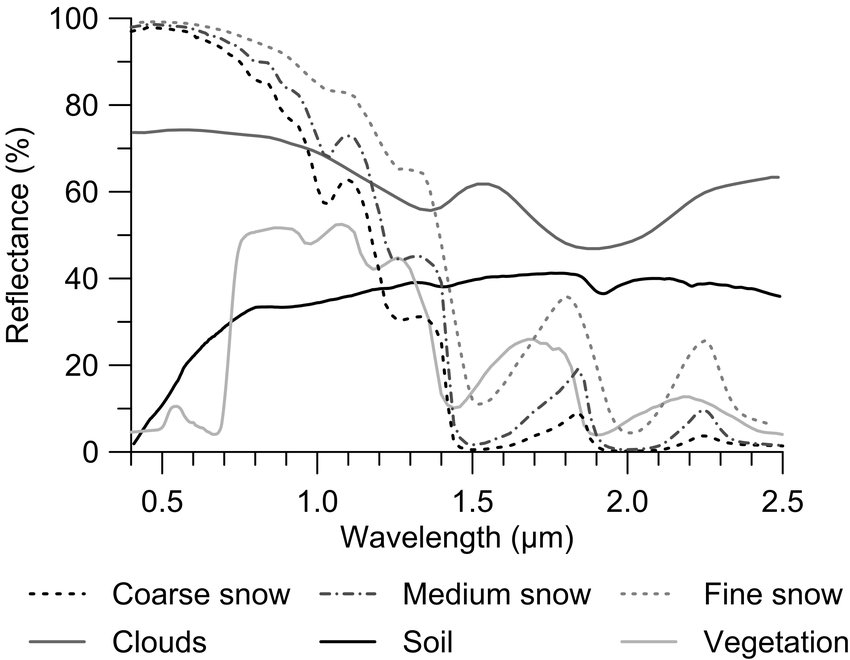
\includegraphics[scale=3]{snow_clouds_reflectance.jpg}
        \captionof{figure}{Spectral Reflectance of Snow, Soil, and Vegetation (\cite{snowcover})\label{fig:reflectance}}
    \end{center}
    \bigskip

    Using MODIS as an example, MODIS band 4 (centered on .555$\mu$m) and band 6 (centered on 1.24$\mu$m) are used to calculate the NDSI (\cite{snowcover}). However, the NDSI's reliance on only two bands leaves it vulnerable to mislabeling pixels, namely cirrus clouds and areas within the tropics. To combat false positives in areas that cannot possibly have snow, MODIS uses a specific value derived from the brightness temperature difference, $BT_11 - BT3.9$(\cite{atbd_snow}), which is stored in Bit 19 of the MODIS' cloud mapping product. Therefore, to remove false positives in tropical areas, the snow cover product also requires collection that either allows a similar calculation or similar collection (MODS band 22: 3.9$\mu$m, MODUS band 31: 11.03$\mu$m). To combat mislabeling pixels as Cirrus clouds, MODIS band 26 (centered on 1.38 $\mu$m) is utilized, and the output is also available in MODIS' cloud mapping product. Using all of the bands, MODIS obtains an error expected to be around 7.5 percent (\cite{snowcover}) with a 1000m resolution and a 2-day temporal resolution. The ECV for snow cover requires a threshold resolution of 48 hours (2 days), a horizontal resolution of 1000 m, and the threshold time delivery for the product to be 240 hours (10 days) (\cite{2022ecvs}). The ECV's goals are more ambitious, requiring a spatial resolution of 50 meters with a temporal resolution of 6 hours. Although this ECV's threshold is entirely met by MODIS, the goals are not met by MODIS, but there are other platforms that could be evaluated. 
    
    \pagebreak
    \item \textbf{Identify satellite sensor specification for fire, aerosol, Land Surface Temperature (LST), and vegetation monitoring from space. Discuss satellite, sensor name, orbit, swath, spatial resolution, band center and width, spectral radian, required Signal-To-Noise (SNR) Ratio or Noise-equivalent temperature difference (NE($\Delta$)T).}

    \bigskip
    Launched in 1999 and 2002, Terra and Aqua satellites orbit Earth in a near polar orbit with the Moderate Resolution Imaging Spectrometer (MODIS) sensor (\cite{qubook}). MODIS was designed to facilitate monitoring of numerous geophysical parameters with its' 36 bands and scan swath of 2,330 kilometers, which extends 10 kilometers at nadir (\cite{qubook}). Using MODIS collected-data, NASA produces a variety of products, such as Thermal Anomalies - Active Fires, Aerosol, Vegetation Indices, and Land Surface Temperature and Emissivity products (\cite{modwebsite}). Each product implements a unique algorithm and is reliant on different MODIS bands. For the Thermal Anomalies - Active Fires product, the algorithm is reliant on bands 1, 2, 7, 21, 22, 31, and 32 (\cite{modisfireatbd}). MODIS Bands 21, 22, and 31 all assist with active fire detection; however, bands 21 and 22 only support fire detection within the algorithm. Within the MODIS Level 1 ATBDs, Band 21 is listed as primarily supporting fire detection and its' calibration is discussed heavily due to special circumstances (\cite{modis1batbd}). Bands 1, 2, 7, and 32 are used to create cloud masks, identify sun glint or bright surfaces, or assist with rejections (\cite{modisfireatbd}). NASA's Aerosol product uses MODIS bands 1-7, as well as band 26 for cirrus correction (\cite{aerosolatbd}). Currently, NASA produces two vegetation index (VI) products using MODIS: (1) the Normalized Difference Vegetation Index (NDVI) and (2) the Enhanced Vegetation Index (EVI). MODIS Bands 1 (250m spatial resolution, ~red) and 2 (250m spatial resolution, NIR) are mentioned to be critical to both VI products. Given that NDVI is calculated using two bands (near infrared and red), this is expected. Combined, the ATBDs for both VI products use bands 1-7 (\cite{modis_veg}). Similar to fire, additional bands are included to assist with cloud masks, atmospheric correction, reflection signatures, etc. Finally, NASA produces two separate LST and emissivity products, MOD11 and MOD21. MOD11 was determined to underestimate the LST in desert regions; however, MOD21 does not experience the same inaccuracies (\cite{mod11_web}). MOD11 remains published due to user's requesting continued publication; however, MOD21 is considered to provide greater worldwide accuracy (\cite{mod11_web}). Depending on the specific LST product, bands 20, 22, 23, 29,  31, 32, and 33 may be used (\cite{modis_lst21}). MOD11 uses MODIS bands 20, 22, 23, 29, 31-33; however, MOD21 only uses MODIS thermal infrared bands 29, 31, and 32 (\cite{modis_lst21}).

    The exact specifications for the bands are listed in Table~\ref{Tab:Tcr}, which matches the requirements listed in the ATBD. 
    \begin{center}
    \pagebreak
    {\setstretch{1.0} % force the table onto one page
    \captionof{table}{MODIS Bands (\cite{qubook})\label{Tab:Tcr}}
    \begin{tabular}{| c | c | c | c | c | c | c | }
        \hline
        Band & Width($\mu$m) & Center($\mu$m) & Spatial Res(m) & Spectral Radiance & SNR & NE$\Delta$T(K) \\ [.5ex]
        \hline
        1 & .62 - .67 & .645 & 250 & 21.8 & 128 & -  \\
        2 & .841 - .876 & .8585 & 250 & 24.7 & 201 & -  \\
        \hline
        3 & .459 - .479 & .469 & 500 & 35.3 & 243 & -  \\
        4 & .545 - .565 & .555 & 500 & 29.0 & 228 & - \\
        5 & 1.230 - 1.250 & 1.24 & 500 & 5.4 & 74 & - \\
        6 & 1.628 - 1.652 & 1.64 & 500 & 7.3 & 275 & - \\
        7 & 2.105 - 2.155 & 2.13 & 500 & 1.0  & 110 & - \\
        \hline
        8 & .405 - .420 & .4125 & 1000 & 44.9 & 880 & - \\
        9 & .438 - .448 & .443 & 1000 & 41.9 & 838 & - \\
        10 & .483 - .493 & .488 & 1000 & 32.1 & 802 & - \\
        11 & .526 - .536 & .531 & 1000 & 27.9 & 754 & - \\
        12 & .546 - .556 & .551 & 1000 & 21.0 & 750 & - \\
        13 & .662 - .672 & .667 & 1000 & 9.5 & 910 & - \\
        14 & .673 - .683 & .678 & 1000 & 8.7 & 1087 & - \\
        15 & .743 - .753 & .748 & 1000 & 10.2 & 586 & - \\ 
        16 & .862 - .877 & .8695 & 1000 & 6.2 & 516 & - \\
        \hline
        17 & .890 - .920 & .905 & 1000 & 10.0 & 167 & - \\
        18 & .931 - .941 & .936 & 1000 & 3.6 & 57 & - \\
        \hline
        19 & .915 - .965 & .94 & 1000 & 15.0 & 250 & - \\
        20 & 3.660 - 3.840 & 3.75 & 1000 & .45 & - & .05 \\
        21 & 3.929 - 3.989 & 3.959 & 1000 & 2.38 & - & 2.0 \\
        22 & 3.929 - 3.989 & 3.959 & 1000 & .67 & - & .07 \\
        23 & 4.020 - 4.080 & 4.05 & 1000 & .79 & - & .07 \\
        24 & 4.433 - 4.498 & 4.4655 & 1000 & .17 & .25 & - \\
        25 & 4.482 - 4.549 & 4.5155 & 1000 & .59 & .25 & - \\
        \hline
        26 & 1.360 - 1.390 & 1.375 & 1000 & 6 & 150 & - \\
        \hline
        27 & 6.535 - 6.895 & 6.715 & 1000 & 1.16 & .25 & - \\
        28 & 7.175 - 7.475 & 7.325 & 1000 & 2.18 & .25 & - \\
        29 & 8.400 - 8.700 & 8.55 & 1000 & 9.58 & .05 & - \\
        \hline
        30 & 9.580 - 9.880 & 9.73 & 1000 & 3.69 & .25 & - \\
        \hline
        31 & 10.780 - 11.280 & 11.03 & 1000 & 9.55 & .05 & - \\
        32 & 11.770 - 12.270 & 12.02 & 1000 & 8.94 & .05 & - \\
        33 & 13.185 - 13.485 & 13.335 & 1000 & 4.52 & .25 & - \\
        34 & 13.485 - 13.785 & 13.635 & 1000 & 3.76 & .25 & - \\
        35 & 13.785 - 14.085 & 13.935 & 1000 & 3.11 & .25 & - \\
        36 & 14.085 - 14.385 & 14.235 & 1000 & 2.08 & .35 & - \\
        \hline
    \end{tabular}
    } % end single line
\end{center}
    \pagebreak
    \item \textbf{Review an ATBD and An Introduction to Atmospheric Radiation Chapter 1. Write a summary about Blackbody law applications on the associated ATBD.}
    
    Chapter 1 discusses 4 blackbody radiation laws: Planck's, Stefan-Boltzmann, Wien's Displacement, and Kirchoff's. Planck's law represents the intensity of a blackbody at a specific temperature and wavelength. The Stefan-Boltzmann Law provides the total intensity of a blackbody, and Wien's Displacement provides the wavelength where the intensity of blackbody radiation is the strongest. Lastly, Kirchoff's law states emissivity of a given wavelength is equal to the absorptivity. 

    \bigskip
    NOAA's Visible Infrared Imaging Radiometer Suite (VIIRS) collects data on 22 spectral bands, which vary from .412 $\mu$m to 12.01 $\mu$m. From the Sensor Data Record, VIIRS produces 23 Environmental Data Records (EDRs), which support products such as aerosol monitoring, active fire detection, and sea surface temperature. Reviewing the NOAA ATBD which "provides guidelines for the production of calibrated top of atmosphere (TOA) radiances, calibrated TOA reflectances, and calibrated TOA brightness temperatures from VIIRS Raw Data Records (RDR)", it is clear that blackbody radiation laws are critical to properly performing radiometric calibration (\cite{noaa_atbd}). When conducting pre-launch calibration, Planck's formula is used to validate the Blackbody Calibration Source (BCS) to validate it is a near-perfect blackbody. Similarly, Planck's Function is used alongside the On-Board Calibrator Blackbody (OBCBB) to ensure that it has an emissivity of ~1.0 (i.e., almost a perfect blackbody). When calculating the irradiance for the field stop from an emissive source, Planck's Function is one of the four factors listed (\cite{noaa_atbd}). 


    \item \textbf{An infrared scanning radiometer aboard a meteorological satellite measures the outgoing radiation emitted from the earth's surface in the 10 $/mu$m window region. Assuming that the effect of the atmosphere between the satellite and the surface can be neglected, what would be the temperature of the surface if the observed radiance at 10 $\mu$m is \(9.8 W m^{-2}\) $\mu$\(m^{-1} sr^{-1}\).} 
    
    Since we have the observed radiance (\(9.8 W m^{-2}\) $\mu$\(m^{-1} sr^{-1}\)) and central wavelength (10 $\mu$m) but desire Temperature, the inverse Planck function can be used. The answer is 299.2 K.

    \( T = (C_2/(ln((C_1/I_{\lambda})+1)))\), where

    \( C_2 = (hc)/(k\lambda)\) is the second radiation constant and

    \( C_1 = 2hc^2\lambda^{-5}\) is the first radiation constant

    \begin{lstlisting}
        import math
        h = 6.626068 * (10**-34) #joules/sec
        c = 2.997925 * (10**8) #m/s
        K = 1.38066 * (10**-23) #joules/degree
        lambda_ = 10**-5 # meters
        C1 = 2*h*c*c*(lambda_)**-5 #Watts / 
        C2 = (h*c)/(lambda_*K)
        I = 9.8 / (10**-6) # divide by 1 * 10^-6 to convert mum to meters to be compatible with K1
        
        print(C1) #1191042919.6552804 W m^-3 sr^-1
        print(C2) #1438.7651491967606 K
        
        T = C2/math.log((C1/I) + 1)
        
        print(T) #299.21931528251974
        
        
    \end{lstlisting}

    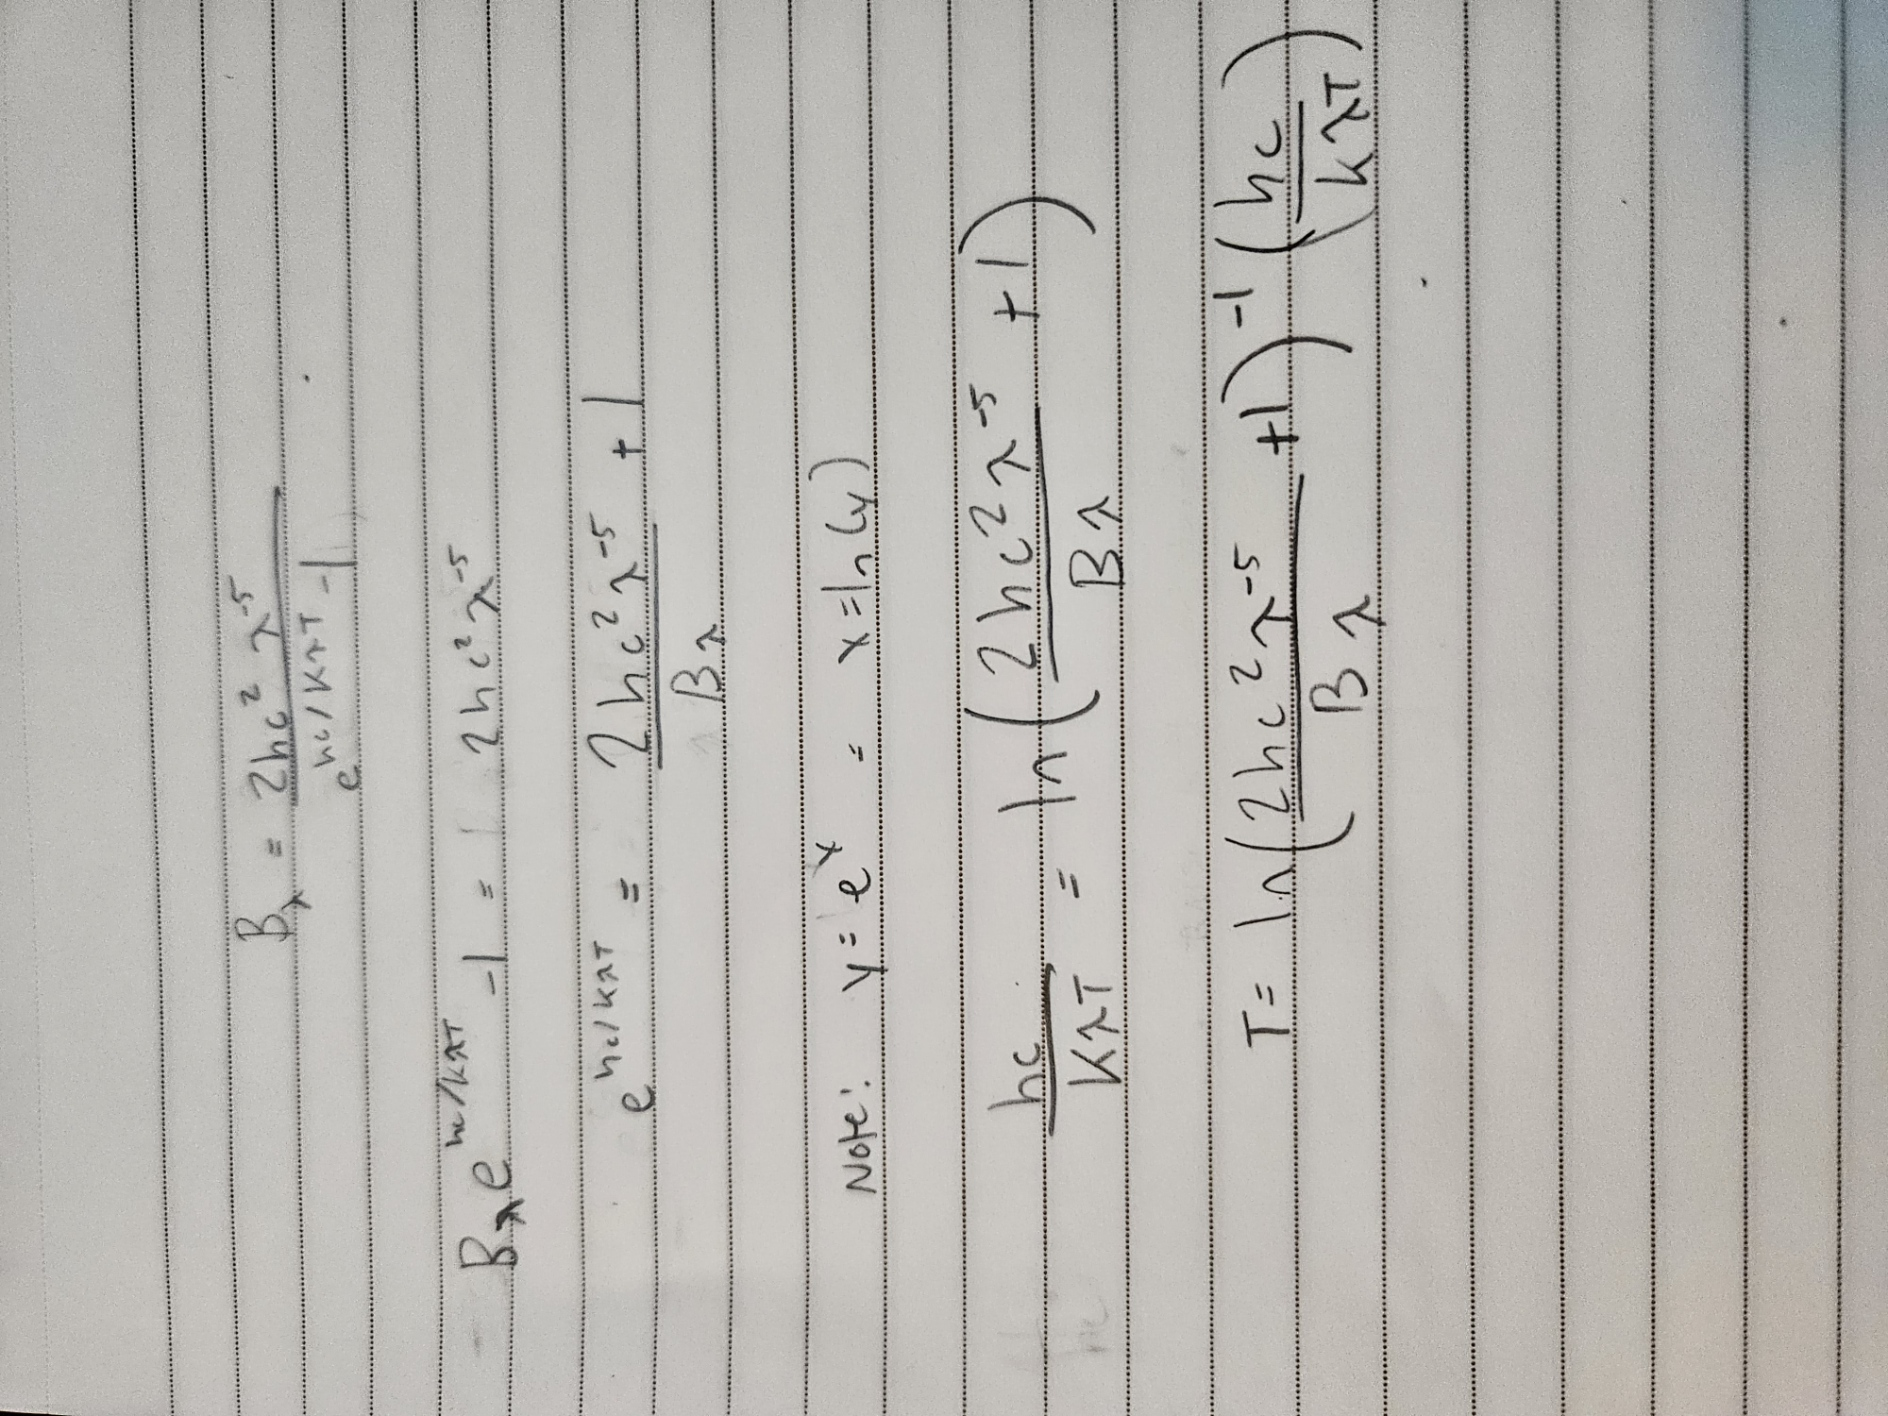
\includegraphics[scale=.3, angle=-90]{planckreversal.jpg}

\end{enumerate}
%\cite{qubook}
%\cite{modisfireatbd}
\pagebreak
\bibliographystyle{apacite}
\bibliography{refs}
\end{document}